\documentclass[10pt,a4paper]{article}

\usepackage[margin=1.5cm]{geometry}
\usepackage[UKenglish]{babel}
\usepackage{enumitem}
\usepackage{fancyhdr}
\usepackage{graphicx}

\pagestyle{fancy}
\lhead{T Davies, A Fahie, A Fairbairn, A Free, J Mansfield, R Tucker, M Walker}
\chead{}
\rhead{GPIG-C}
\cfoot{}

\setlist{nolistsep} % Reduces lots of white space around lists

\renewcommand{\headrulewidth}{0.4pt} % Add rules below header
\renewcommand{\footrulewidth}{0.4pt}

\begin{document}

\title{\vspace{-1cm}GPIG-C Initial Report}
\author{}
\date{\vspace{-1cm} Friday, 25th October}
\maketitle
\thispagestyle{fancy} % Make sure header and footer appear on the front page

\section{Introduction}
\subsection{Single Statement of Need}
This project aims to deliver a tailorable Health and Usage Monitoring System (HUMS), tailorable to multiple target domains. The target for the system is any consumer needing to collect, store, analyse and report data from one or more data input clients.
\subsection{Intended Audience of this Document}
The intended audience of this document are both the developers and the customer. The document is structured in a manner which will interest all concerned parties. Requirements will follow the introduction, followed by use cases, a review of possible solutions and a risk register.

\section{Use cases}


\section{Requirements}
For this project, requirements have been divided into three categories, functional, non-functional and constraint. The requirements have been engineered such that each falls into one of those three categories, this prevents them from becoming too complex. Each requirement has been structured as simply and concisely as possible and been worded in such a way as to avoid ambiguity. The requirements represent the problem to be solved and serve as a contract between us, as the development team, and the customer. All requirements have therefore been checked with the customer to ensure the system described is the system they envisioned.\\
The functional requirements detail what inputs, behaviour and outputs the system must provide. The non-functional requirements specify the qualities of the system as opposed to its behaviour. Constraint requirements are those that apply to the entire system, including any constraints on the environment the system can be used in and any timing constraints. In order to ensure all requirements are verifiable, appropriate testing procedures have been included.

\subsection{Functional requirements}

\subsection{Non-functional requirements}

\subsection{Constraint requirements}

\section{Possible solutions}

\subsection{Proposed solution}

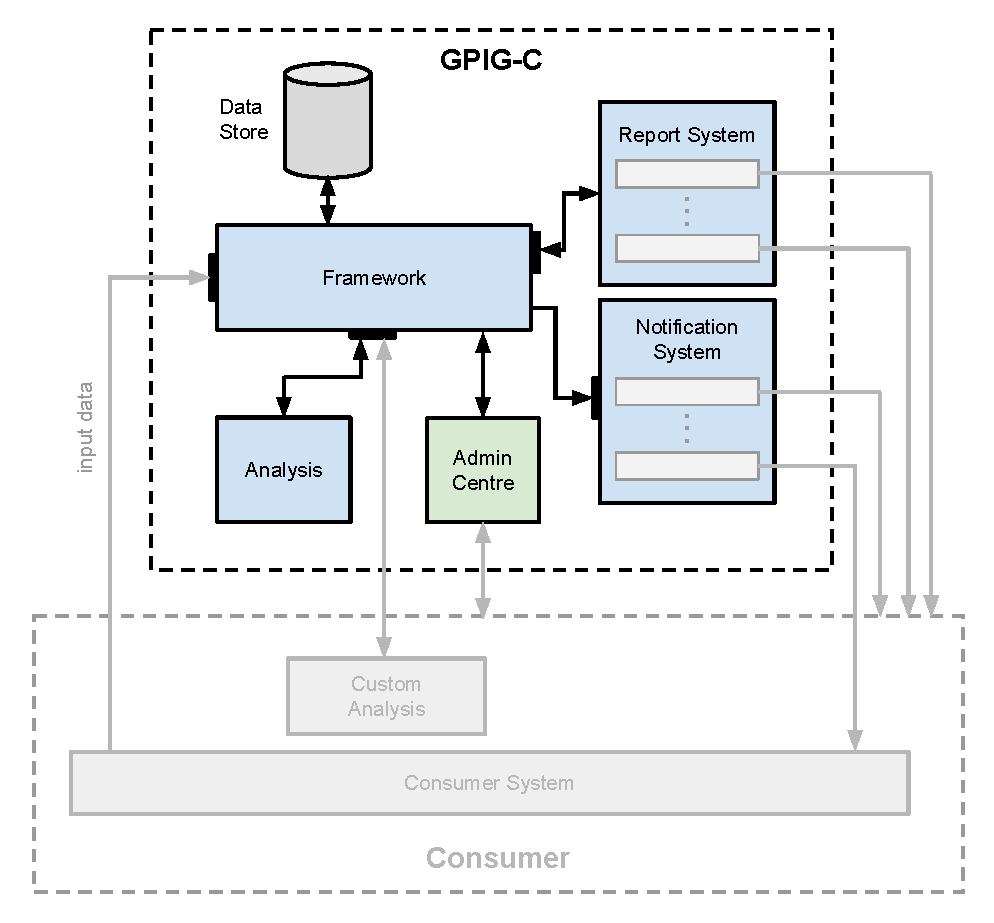
\includegraphics[width=0.75\textwidth]{system-architecture.pdf}


\section{Team organisation}

\subsection{Team members}

\subsection{Roles}


\section{Development plan}

\subsection{Software engineering methodology}

\subsection{Schedule}


\section{Risk register}


\section{Customer communication}


\end{document}
